% Standalone LaTeX version of docs/eval_summary.md.
% Self-contained (no dependency on DS-A2A.tex's macros/preamble) so it
% compiles on its own. All numbers are taken directly from
% evaluation/results/csv/devbench_summary_{qwen2.5-coder-7b,devstral-24b,
% qwen3-coder-30b,pooled}.json; nothing here is projected or invented.
%
% The table below deliberately reports only metrics NOT already shown in
% Figure~\ref{fig:rq1rq2}: the figure gives the per-model breakdown of RQ1
% P1 modes, RQ2 precision, and RQ1 tokens/task; the table gives the pooled
% RQ1 canary/acceptance results, RQ2 recall and RQ2 tokens-per-change, and
% the RQ3 results, none of which the figure depicts.

\documentclass[11pt]{article}

\usepackage[margin=1in]{geometry}
\usepackage{graphicx}
\usepackage{booktabs}
\usepackage{multirow}
\usepackage{amsmath}
\usepackage{hyperref}

\newcommand{\tool}{AgentM2M}

\title{AgentM2M Preliminary Evaluation --- Summary}
\author{}
\date{}

\begin{document}
\maketitle

\noindent\textit{Condensed from \texttt{sec\_eval\_revised.tex}. All
numbers below are taken directly from
\texttt{evaluation/results/csv/devbench\_summary\_\{qwen2.5-coder-7b,
devstral-24b,qwen3-coder-30b,pooled\}.json}; nothing here is projected or
invented.}

\section*{Prototype and benchmark}

The prototype executes coordination rules over EMF-compatible metamodels
with pluggable LLM backends. The evaluated pipeline (\tool{}) uses four
view metamodels and four hand-offs between agent roles. We evaluate
against DevBench, the closest public benchmark available: its
repositories ship with a PRD, a UML/architecture design, and executable
acceptance/unit tests. These map onto the prototype's own views ---
$M_{\mathit{req}}$ (PRD $\to$ UserStory/Criterion), $M_{\mathit{arch}}$
(UML $\to$ Component/Operation) --- and DevBench's own unmodified tests
serve as the oracle. Of DevBench's 22 repositories across four languages,
we target the 10 Python ones, since the prototype's validators
(\texttt{python\_compiles}, \texttt{run\_pytest\_oracle}) are
Python-specific. Given measured per-repository latency (roughly 46 tok/s
for \texttt{qwen2.5-coder:7b}, 15 tok/s for \texttt{devstral:24b}, 45
tok/s for \texttt{qwen3-coder:30b}), only the smallest repository,
\texttt{chakin} (9 operations, including 5 seeded canary operations), has
complete runs across all three models and configurations so far.

\section*{Research questions}

Three configurations are compared under identical roles, prompts, and
LLM: \textbf{free-text} hand-offs, a \textbf{PatchBoard-style shared
schema} (which validates each write but does not relate views to each
other), and \textbf{\tool{}}. Each runs on three open-weight models
spanning small, agentic-specialist, and large points on the current
open-model landscape: \texttt{qwen2.5-coder:7b}, \texttt{devstral:24b},
and \texttt{qwen3-coder:30b}.

\begin{itemize}
\item \textbf{RQ1 (fidelity).} Does \tool{} reduce coordination failure
modes (MAST ``P1'' modes)? We measure canary retention (5 seeded
operations with their own tests, absent from every real repository so
memorization cannot help), P1 modes per trace via a MAST-annotator
approximation, and DevBench's own acceptance pass rate.
\item \textbf{RQ2 (change).} Under three injected PRD changes per
repository (tighten/add/remove a criterion), what are the precision and
recall of \tool{}'s change-impact operator against the declared-footprint
impact set --- the one operation each changed UserStory targets by
construction of the rule set? We compare against an LLM asked to list
affected artifacts (free text) and against regenerating everything
(shared schema), also counting tokens.
\item \textbf{RQ3 (evolution).} Can a higher-order transformation alone
add a Security Reviewer mid-run, and at what cost versus manual
rewiring? We report glue-code lines changed and the share of
pre-existing operations retroactively covered.
\end{itemize}

\section*{Results}

On \texttt{chakin}, \textbf{no} model/configuration pair (9 of 9) retained
any canary or passed the real acceptance test --- a genuine, if
unencouraging, result at this scale (a scripted backend that returns
correct canary bodies passes 5/5 through the same code path, confirming
the harness works). MAST P1 modes gave a mixed, model-dependent signal:
\texttt{qwen2.5-coder:7b} showed 0 P1 modes in all three configurations;
\texttt{devstral:24b} showed \emph{more} P1 modes for \tool{} (3) than
free text (2) or shared schema (1); \texttt{qwen3-coder:30b} showed
\emph{fewer} P1 modes for \tool{} (0) than free text (2), matching shared
schema (0). Averaged, P1 modes per trace were 1.33 (free text), 0.33
(shared schema), and 1.00 (\tool{}): \tool{} sits between the two
baselines, and the ranking flips by model.

RQ2 was the one metric where all three models agreed exactly: \tool{}
reached recall 1.00 and precision 1.00 on all 9 real trials (3 models
$\times$ 3 injected changes), never missing and never over-including. The
baselines did not hold as steady --- shared schema was recall 1.00 /
precision 0.23 identically across models (it regenerates everything, as
expected), while free-text precision varied non-monotonically with model
size: 1.00 (\texttt{qwen2.5-coder:7b}), 0.75 (\texttt{devstral:24b}), 0.23
(\texttt{qwen3-coder:30b}, indistinguishable from ``regenerate
everything''). \tool{} cost more tokens per RQ1 task (25.5k mean) than
free text (14.9k) or shared schema (4.8k), and 34.0k tokens per RQ2
change versus 0.23k (free text) and 0k (shared schema, no LLM calls).

RQ3 was deterministic and identical across all three models: the added
Security Reviewer covered all 9 pre-existing operations (100\%
retroactive coverage) for 7 lines of glue code, versus an estimated 22
lines for hand-written baseline retrofits.

\begin{figure}[t]
\centering
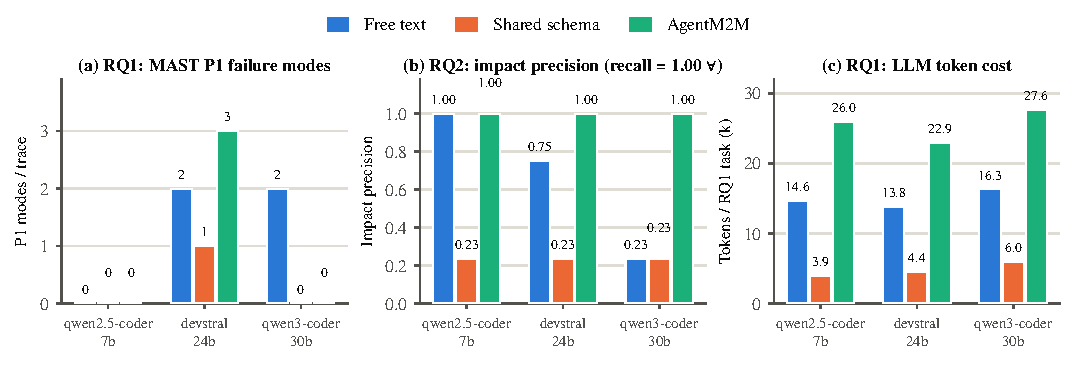
\includegraphics[width=\textwidth]{../evaluation/results/figures/devbench_rq1_rq2_per_model.pdf}
\caption{Per-model breakdown, $n{=}1$ repository (\texttt{chakin})
$\times$ 3 models. (a) MAST P1 modes per trace: the sign of \tool{}'s
effect flips by model (worse with \texttt{devstral:24b}, better with
\texttt{qwen3-coder:30b}, no signal with \texttt{qwen2.5-coder:7b}). (b)
RQ2 impact precision (recall $=1.00$ for every model/configuration):
\tool{} holds precision $1.00$ for all three models while free text is
non-monotonic in model size. (c) LLM tokens per RQ1 task: \tool{} costs
more than either baseline at this scale.}
\label{fig:rq1rq2}
\end{figure}

Table~\ref{tab:pooled} complements the figure with the pooled metrics the
figure does not plot: RQ1 canary retention and acceptance pass rate
(both 0\% everywhere, so not worth a per-model panel), RQ2 recall
(identically 1.00 across every model/configuration), RQ2 tokens per
change, and the RQ3 results, which have no per-model spread at all since
all three models produced the same outcome.

\begin{table}[t]
\centering
\caption{DevBench pilot results on \texttt{chakin}, pooled over the 3
models (\texttt{qwen2.5-coder:7b}, \texttt{devstral:24b},
\texttt{qwen3-coder:30b}). Metrics already broken out per model in
Figure~\ref{fig:rq1rq2} (P1 modes per trace, RQ2 precision, RQ1 tokens per
task) are omitted here to avoid duplicating the figure.}
\label{tab:pooled}
\begin{tabular}{@{}llccc@{}}
\toprule
& Metric & Free text & Shared schema & \tool{} \\
\midrule
\multirow{2}{*}{RQ1} & Canary retention (\%) & 0.0 & 0.0 & 0.0 \\
                     & Acceptance pass (\%)  & 0.0 & 0.0 & 0.0 \\
\multirow{2}{*}{RQ2} & Impact recall          & 1.00 & 1.00 & 1.00 \\
                     & Tokens per change (k)  & 0.23 & 0.00 & 34.01 \\
\multirow{2}{*}{RQ3} & Glue lines changed        & -- & -- & 7 vs.\ 22 (manual) \\
                     & Retroactive coverage (\%) & -- & -- & 100.0 \\
\bottomrule
\end{tabular}
\end{table}

\section*{Discussion}

Canary retention was 0\% everywhere, so RQ1 is \textbf{inconclusive} at
this sample size --- a paired bootstrap isn't computable with one
repository, and a null result cannot distinguish ``no effect'' from
``underpowered.'' RQ2 is the strongest result: recall and precision were
both 1.00 for \tool{} on every real trial, following structurally from
the change-impact operator's design rather than generation quality. RQ3
behaved identically across models for the same structural reason.

The clearest limitation is scale: a \textbf{single-repository (n=1),
3-model pilot}, not a statistically powered comparison. The MAST
annotator is our own approximation of an unreleased tool and, being the
same class of model it evaluates, may be miscalibrated for \tool{}'s
non-conversational, per-operation transcript shape. \tool{}'s token cost
is higher than either baseline at generation time, so its practical case
rests on the RQ2 change-time savings above, not cheaper initial
generation. Converting token counts into an energy estimate remains
pending.

\end{document}
